Nella fase 3 hanno luogo le seguenti attività:
\begin{itemize}
	\item normazione: modifiche alle \textit{NormeDiProgetto\_v2.0.0} secondo quanto segnalato alla Revisione di progettazione. Si procede poi con il suo incremento;
	\item pianificazione della qualifica: modifiche al \textit{PianoDiQualifica\_v2.0.0} secondo quanto segnalato alla Revisione di progettazione. Si procede poi con il suo incremento;
	\item pianificazione delle attività: modifiche al \textit{PianoDiProgetto\_v2.0.0} secondo quanto segnalato alla Revisione di progettazione;
	\item progettazione in dettaglio e Product Baseline: questa attività presenta la baseline architetturale del prodotto tramite diagrammi delle classi e di sequenza, mostrando coerenza con quanto mostrato nel PoC;
	\item codifica: realizzazione del prodotto;
	\item verifica per il colloquio: verifica del codice scritto in vista del colloquio Agile con il committente;
	\item colloquio: viene effettuato il colloquio con il committente;
	\item redazione manuali: redazione \textit{ManualeUtente\_v2.0.0} e \textit{ManualeSviluppatore\_v2.0.0};
	\item incremento progettazione e codifica: in base a alle segnalazioni ricevute al colloquio con il committente viene eseguito l'eventuale incremento;
	\item incremento della pianificazione delle attività: viene aggiornato il \textit{PianoDiProgetto\_v2.0.0} con il consuntivo pre-finale;
	\item verifica per la consegna: vengono verificati tutti i documenti e il Product Baseline con la relativa codifica;
	\item consegna del materiale in ingresso;
	\item preparazione alla presentazione.
\end{itemize}

\begin{figure}[h]
	\centering
	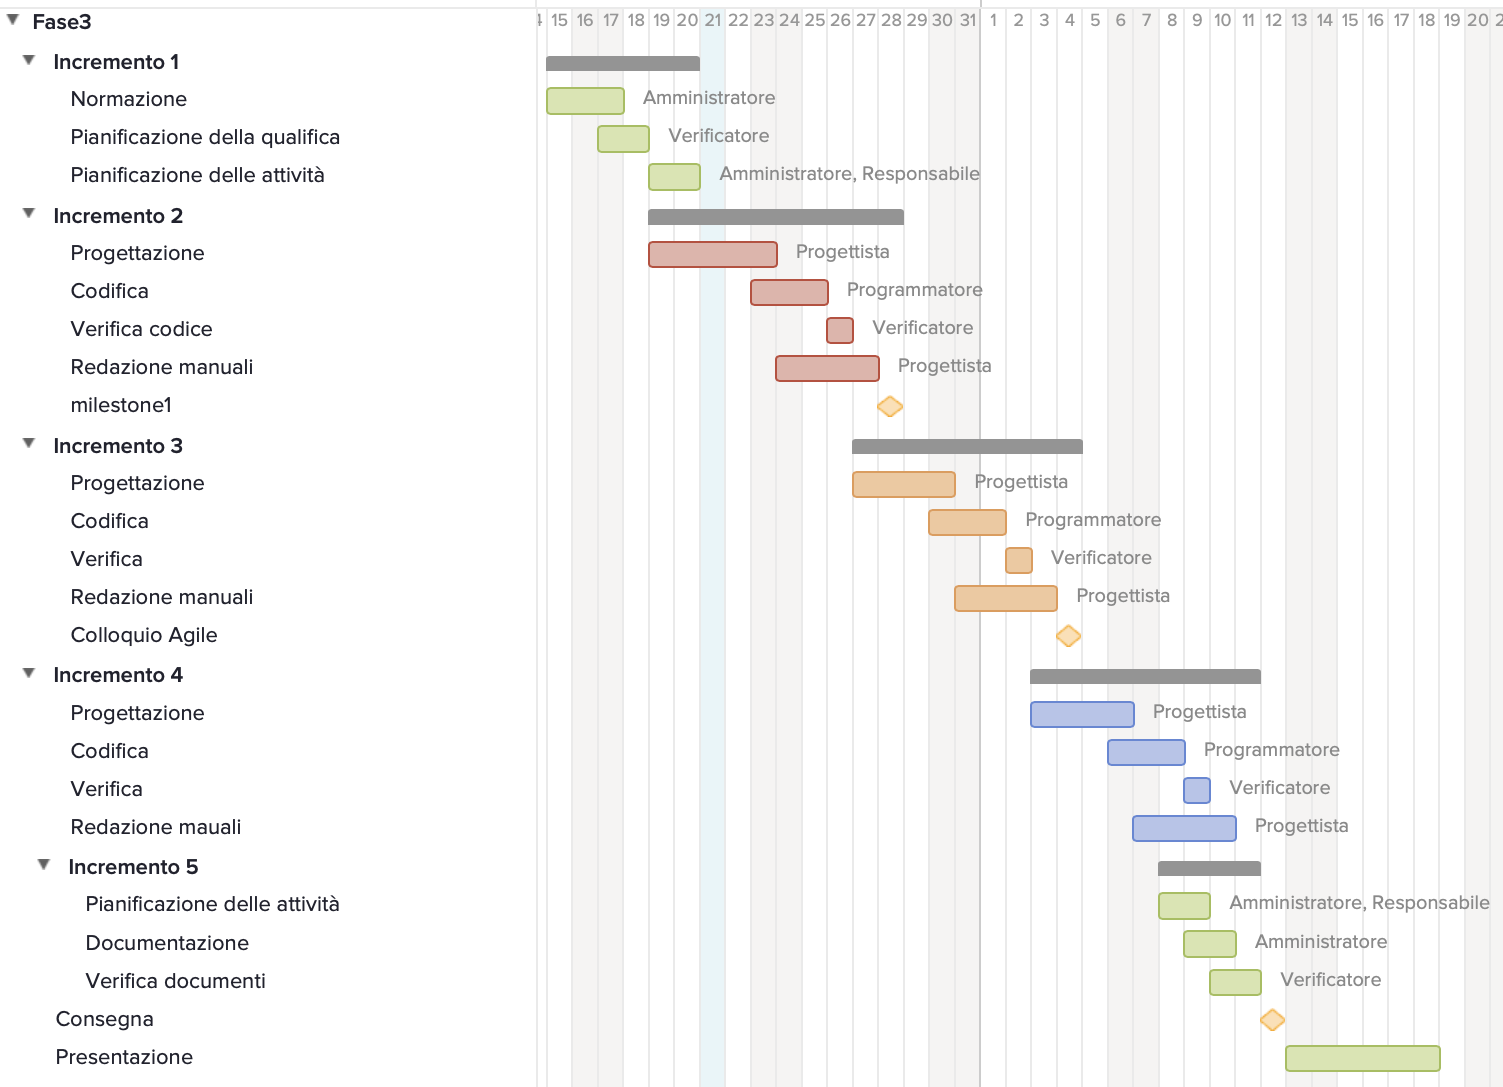
\includegraphics[scale=0.70]{images/fase3.png}
	\caption{Diagramma di Gantt riguardante la fase 3}
\end{figure}